\chapter{System Design and Implementation}\label{ch:implementation}
The system pipeline\footnote{See footnote on page~\pageref{foot:pipe}} consists of three separate processes:
data preprocessing~\ref{sec:data-preprocessing}, feature extraction~\ref{sec:feature-extraction} and
evaluation~\ref{sec:evaluation}.

The system is implemented in \textit{Python} programming language.
Libraries \textit{NumPy} and \textit{PyTorch} are being extensively used throughout the whole pipeline.

\section{Data Preprocessing}\label{sec:data-preprocessing}
\begin{wrapfigure}[7]{r}{0pt}
    \centering
    \raisebox{0pt}[\dimexpr\height-0.831\baselineskip\relax]{%
    \begin{forest}
        for tree={
        font=\ttfamily,
        grow'=0,
        child anchor=west,
        parent anchor=south,
        anchor=west,
        calign=first,
        edge path={
        \noexpand\path [draw, \forestoption{edge}]
        (!u.south west) +(7.5pt,0) |- node[fill,inner sep=1.25pt] {} (.child anchor)\forestoption{edge label};
        },
        before typesetting nodes={
        if n=1
        {insert before={[,phantom]}}
        {}
        },
        fit=band,
        before computing xy={l=15pt},
        }
        [dataset
        [name1
        [image1\_128x128.jpg]
        [image2\_128x128.jpg]
        [image3\_128x128.jpg]
        ]
        [name2
        [image1\_128x128.jpg]
        [image2\_128x128.jpg]
        ]
        [\ldots]
        ]
    \end{forest}
    }
    \caption{Standard image dataset format}
    \label{fig:dataset}
\end{wrapfigure}
The goal of preprocessing is to convert the input dataset~\ref{subsec:dataset-description} to a standard format.
The standardized dataset consists of directories with each directory representing one identity/label.
In these directories there are images corresponding to the identity.
In this case, the images contain faces in different positions.

The desired format is visualized in figure~\ref{fig:dataset}.

\subsection{Dataset Description}\label{subsec:dataset-description}
The input dataset consists of 15 videos and the same amount of annotation files in \textit{json}\footnote{An
open-standard file format that uses human-readable text to transmit data objects consisting of attribute–value pairs
and array data types.} format.

In every annotation file there is a dictionary object, where key is a name and value is a list of detections.
Every detection contains information about frame and the position of the face.
This information is used to transform the dataset to standardized format.
The reference face position was selected by human.
Because of that, the geometry of the area is not always consistent which significantly decreases the model performance.
For this reason, as is described in the following section~\ref{subsec:preproalgo}, this reference position is not
used directly in the algorithm.

\subsection{Preprocessing Algorithm}\label{subsec:preproalgo}
Before the presentation of the algorithm it is necessary to define "Intersection over Union (IoU)."
As the name implies IoU is computed as a fraction with intersection area in the numerator and union area in the
denominator (see figure~\ref{fig:iou}).

\begin{figure}[H]
    \centering
    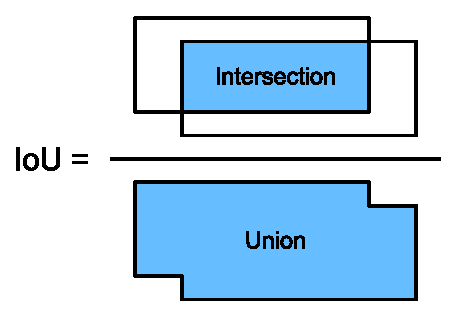
\includegraphics{images/implementation/iou.eps}
    \caption{IoU visualization\cite{IoU}}
    \label{fig:iou}
\end{figure}

The preprocessing algorithm consists of seven steps:
\begin{enumerate}
    \item First I iterate over the annotation files.
    \item Then I iterate over the names and detections within the file.
    \item In the third step I fetch the frame out of the video corresponding to the detection.
    \item Then I detect all the faces in the frame using MTCNN detector.
    The detector returns coordinates of the bounding boxes\footnote{See footnote on page~\pageref{foot:bbox}} and the
    facial landmarks\footnote{Salient regions of the face.}.
    \item I select the detection which meets the following two conditions:
    \begin{enumerate}
        \item has the biggest IoU with the bounding box from the annotation file of all the detections;
        \item the IoU value is at least \textbf{0.5} (This value has been determined experimentally as
        is described in the section~\ref{subsec:detection-mislabelings}.).
    \end{enumerate}
    In case these two conditions are not met for any of the detections the frame is omitted.
    \item Now I perform face frontalization using the facial landmarks from the previous steps and the predetermined
    position of target facial landmarks.
    This is achieved by using the least squares method to find an affine transformation\footnote{A function between
    affine spaces which preserves points, straight lines and planes.} between the two sets of coordinates.
    After the transformation the image geometry is 128x128 and the facial landmarks are in the same position across
    the whole dataset.
    \item In the last step I save the transformed image on the path defined by the standardized dataset format
    (\path{dataset/name/image_128x128.jpg}).
\end{enumerate}

Having the dataset in the desired format we can proceed with feature extraction.

\section{Feature Extraction}\label{sec:feature-extraction}
Feature extraction~\cite{FeEx} is a process of dimensionality reduction by which an initial set of raw data
is reduced to the set of feature vectors.
In this study this process is carried out by feeding the input image $x_i \in \mathbb{R}^{128\times128 }$ to the CNN model.
On the output we retrieve a feature vector $y_i \in \mathbb{R}^{1024}$.

The model used is 18 layer ResNet~\ref{subsec:resnet} which was trained under a supervision of the ArcFace loss.
The training process was not carried out as part of this thesis.
The pretrained model was downloaded from the ArcFace implementation repository~\cite{ArcFacePyTorch}.

\subsection{Feature Extraction Algorithm}\label{subsec:feexalgo}
The feature extraction algorithm consists of 6 steps:
\begin{enumerate}
    \item Initially I will iterate over the images in the dataset.
    \item In the second step I save the image and the flipped version into an array
    with shape $2\times1\times128\times128$.
    \item With this shape, the array can be put on the inputs of ResNet-18.
    \item I retrieve the feature vector on the output.
    \item In the fifth step the vector along with the corresponding label is saved into an array.
    \item Once all the feature vectors are computed, the resulting array is saved using \textit{h5py} module.
\end{enumerate}

In the final array there are 478529 feature vectors.
The whole file is approximately 2 GB in size.

Having the feature vectors computed we can carry out evaluation~\ref{sec:evaluation}.

\section{Evaluation}\label{sec:evaluation}
The system's performance is evaluated on the verification task.
To describe the algorithm in simple words, the task consists of computing cosine distance between every two feature
vectors and deciding, given some threshold, whether the vectors correspond to the same identity ot not.
This computation is carried out for all the threshold values in the specified interval.

The algorithm is described in depth in the following section~\ref{subsec:thresholding-algorithm}.

\subsection{Thresholding Algorithm}\label{subsec:thresholding-algorithm}
First I would like to analyze the algorithm time complexity and memory demands.

As I previously mentioned, it is necessary to compute the distances between every two feature vectors in the dataset.
The number of vector pairs is equal to
\begin{equation}
    N_{pairs} = \frac{n\left(n+1\right)}{2} = \frac{478529\left(478529+1\right)}{2} \approx 114.50 \cdot 10^9,
\end{equation}
where $n = 478529$ is the number of vectors in the dataset.
If we computed all the distances at once using optimized matrix operations we would need at least 460 GB of RAM memory.

Given that the algorithm time complexity is $O(n^2)$ and the big memory demands it was desirable to split the distance
matrix into smaller sub-matrices.
These sub-matrices than could be submitted to different CPU cores to process which significantly reduced the computation
time.
This approach made the use of optimized matrix libraries possible while reducing the excessive memory demands.

There are 5 steps in the parallelized algorithm:
\begin{enumerate}
    \item Initially I generate all the interval pairs.
    \item In the second step I pass the intervals as an argument to the generator function.
    This function returns pairs of slices of the feature vector array and corresponding labels.
    \item Next I pass the generator function as an argument to the \textit{imap} method from \textit{multiprocessing}
    module.
    This method iterates over the generator function and passes the retrieved values to separate processes.
    With this step, parallelized processing is achieved.
    \item In the fourth step the matrix of cosine distances is computed between the two feature vector arrays
    and two label arrays using \textit{cosine\_distances} method from \textit{sklearn} library.
    Computing the matrix for labels allows for simple and efficient comparison of predictions and reference
    values using matrix operations.
    \item Next I convert the matrices to two long vectors.
    \item Now I iterate over the list of threshold values ($\left[ 0, 0.05, 0.10, 0.15, \ldots 2 \right]$).
    \item I apply the threshold to the distances.
    This way I retrieve a vector of binary values.
    \item I use the methods \textit{sum} and \textit{logical\_and} along with elementwise binary value inversion to
    count the number of \textit{true positives (TP)}, \textit{true negatives (TN)}, \textit{false positives (FP)} and
    \textit{false negatives (FN)}.
    \item In the last step I do elementwise summation of the arrays which were returned from the processes.
\end{enumerate}

The output of the algorithm is an array with 200 rows and 4 columns.
The rows correspond to the threshold values; columns to \textit{TP}, \textit{TN}, \textit{FP} and \textit{FN}.

Having all these values accumulated we can proceed with computation of all the relevant metrics.

\subsection{Performance Comparison}\label{subsec:performance-comparison}
In order to evaluate the performance I implemented an algorithm which computes precision~\ref{sec:precision},
recall~\ref{sec:recall} and $F_1$ score~\ref{sec:f-score} on the data from previous section.

In figure~\ref{fig:prft} we can see the progression of these metrics.

\begin{figure}[H]
    \begin{subfigure}{\textwidth}
        \centering
        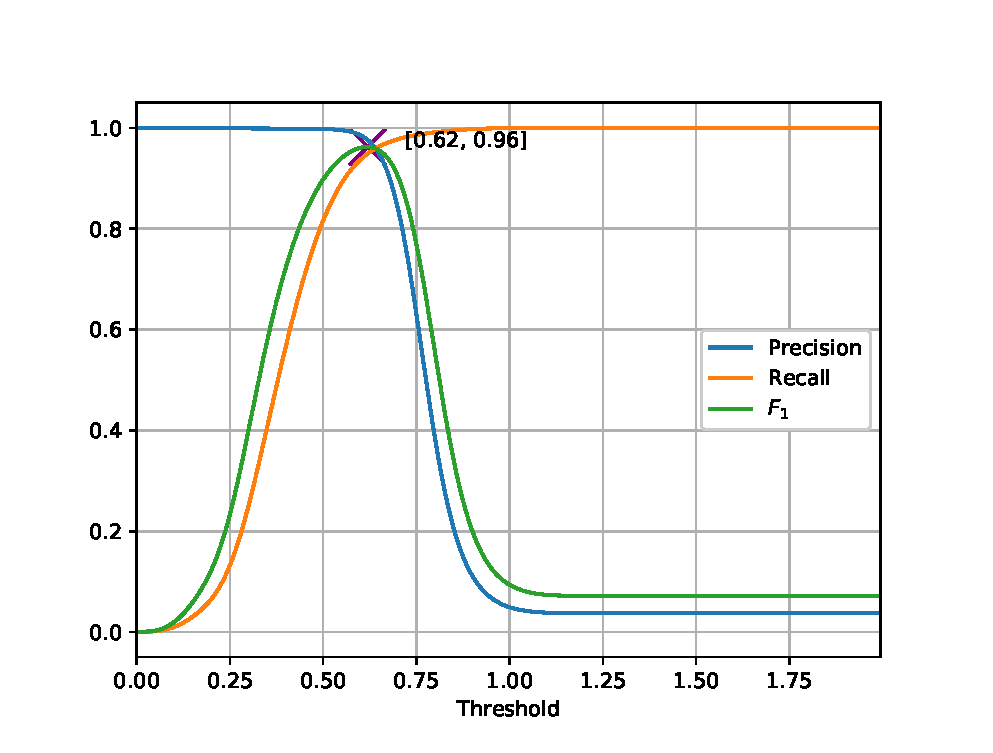
\includegraphics[width=0.95\columnwidth]{images/implementation/prft_fav-128_N1.eps}
        \caption{ResNet-18 trained under a supervision of ArcFace loss function}
        \label{fig:prft_arcface}
    \end{subfigure}%

    \begin{subfigure}{\textwidth}
        \centering
        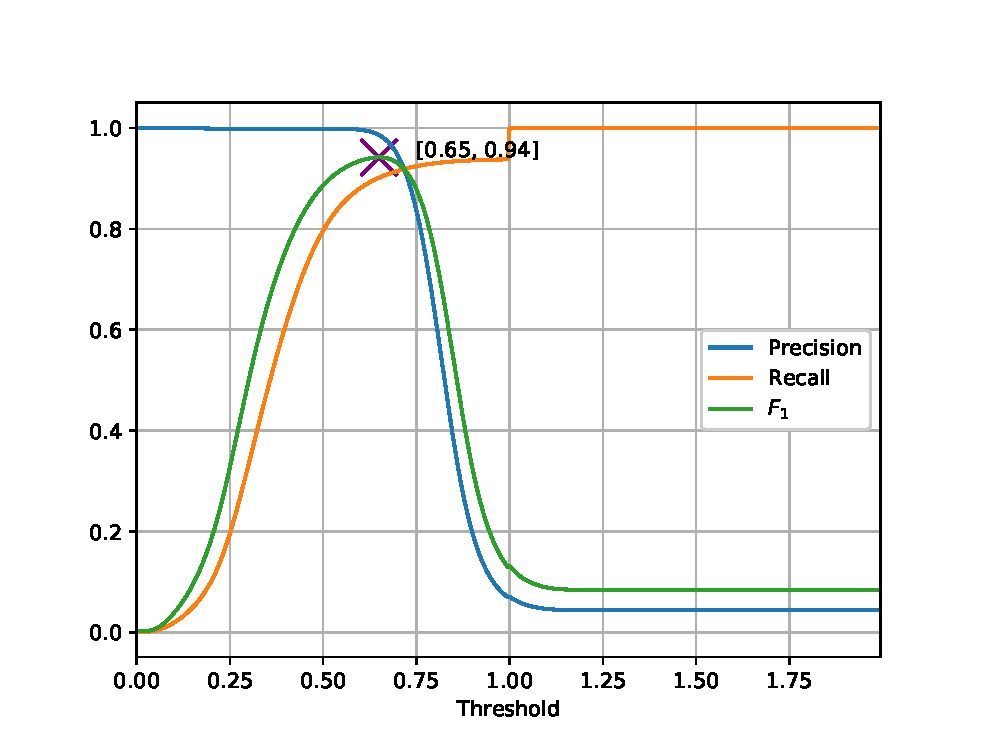
\includegraphics[width=0.95\columnwidth]{images/implementation/prft_eyedea.eps}
        \caption{Commercial system developed by Eyedea Recognition s. r. o.}
        \label{fig:prft_eyedea}
    \end{subfigure}
    \caption{Progression of precision, recall and $F_1$ score with increasing threshold values.}
    \label{fig:prft}
\end{figure}

\subsection{Detection of Mislabelings}\label{subsec:detection-mislabelings}
As I mentioned in the section~\ref{sec:precision}, precision curve can be used to detect incorrect labels in the
dataset.
In figure~\ref{fig:faulty_prft} there are three functions dependent on threshold.

\begin{figure}[H]
    \centering
    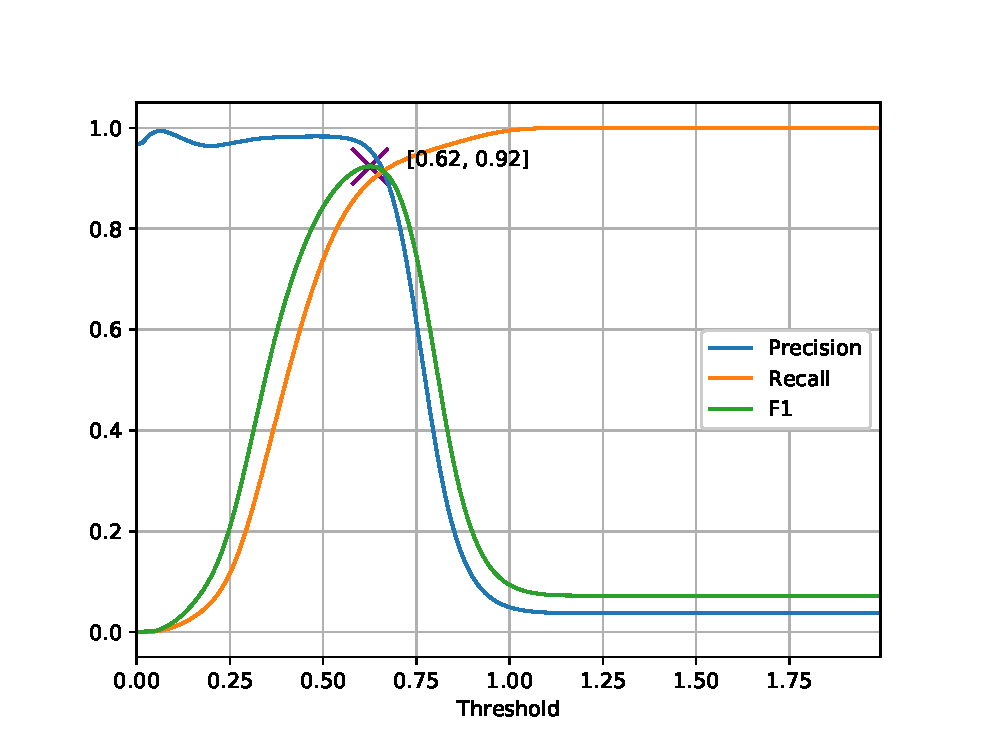
\includegraphics[width=0.95\columnwidth]{images/implementation/faulty_prft.eps}
    \caption{An example of precision curve~\ref{sec:precision} computed on a dataset containing errors.}
    \label{fig:faulty_prft}
\end{figure}

By the definition of precision ($Precision = \frac{TP}{TP+FP}$), there should not be any false positives
for threshold 0 because in such a setting, the system is strongly biased towards false negatives.
With this in mind, value of precision which is not equal to 1 for threshold 0 is a sign that there are either
mislabelings in the dataset or that the whole model is faulty.

\begin{figure}[H]
    \centering
    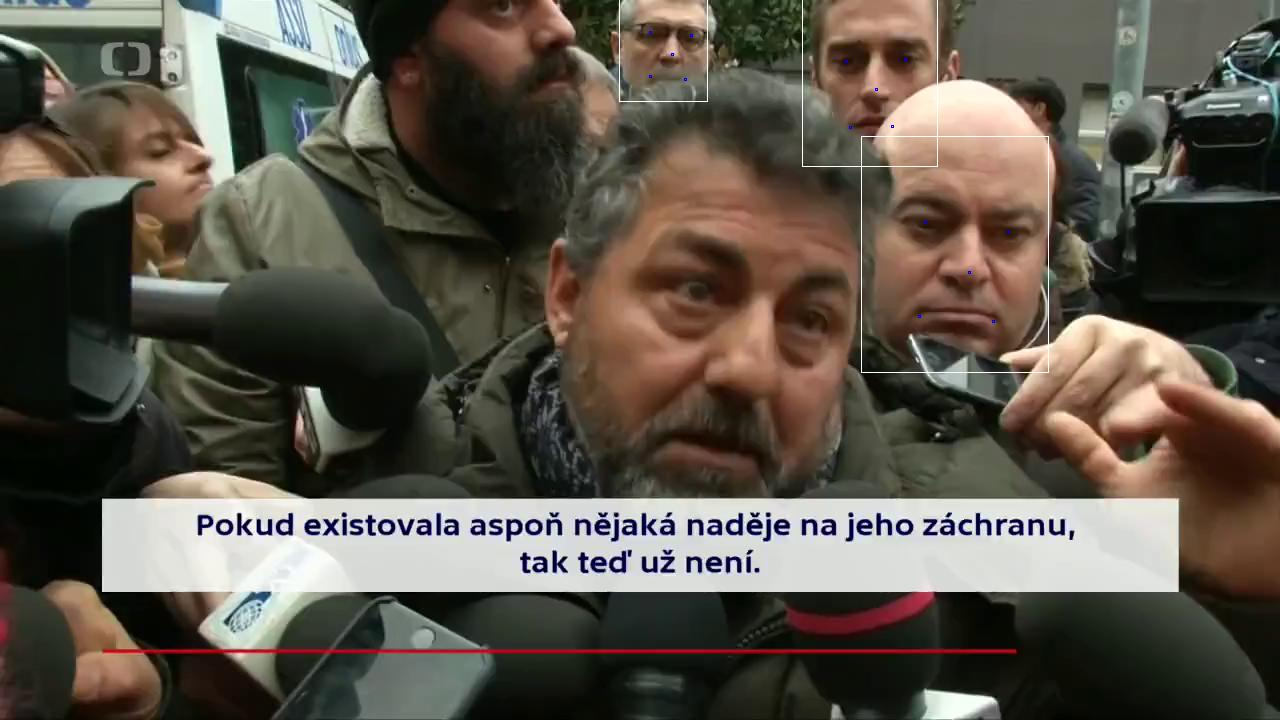
\includegraphics[width=0.9\columnwidth]{images/implementation/faulty_detection.jpg}
    \caption{An example of a faulty detection.}
    \label{fig:faulty_bbox}
\end{figure}

This idea was used extensively during the experimentation.
Figure~\ref{fig:faulty_bbox} is an example of faulty face detection.
Because of the white stripe, the man in the foreground was not detected by the MTCNN detector selecting the bald man
on the right instead.
This led to an error in the dataset and it is the reason why the IoU threshold was put in place during the data
preprocessing~\ref{sec:data-preprocessing}.